\chapter{Introdução}
\label{cap:introducao}

Na última década o crescimento da geração fotovoltaica foi expressivo, de acordo com a IEA (Internetional Energy Agency), a produção global saltou de 32TWh em 2010 para mais de 720 TWh em 2020 \cite{ieasolarpvontrack2020}. No Brasil a geração ainda conta com incentivos fiscais \cite{da2016panorama}, além de um grande potencial ainda subaproveitado, a geração fotovoltaica corresponderá a apenas 2,9\% da produção nacional até 2025 \cite{ONSSIN}. 

Estimativa de potencial de geração fotovoltaica é um tema que já foi muito bem trabalho, mas que continua popular \cite{chin2015cell, jordehi2016parameter, de2017performance}. Os trabalhos levam em consideração a tecnologia utilizada pela célula fotovoltaica e modelos de satélite que visam definir os parâmetros físicos de entrada, tais como radiação, temperatura e velocidade do vento \cite{mueller2009cm, huld2012new, amillo2014new, habte2017evaluation}.

A utilização de técnicas de inteligência artificial aplicadas a este tema tem focado na predição temporal de geração \cite{voyant2017machine, wolff2016statistical, li2016hierarchical}. Este tipo de predição é muito útil levando-se em consideração o sistema elétrico completo de uma região ou país, para balanceamento de oferta e demanda, sendo possível uma programabilidade maior para o operador do sistema elétrico, em relação a adequação do uso de outras fontes de energia.

São encontrados alguns métodos de previsão de energia fotovoltaica na literatura, sendo subdivididos de acordo com o horizonte de previsão \cite{mellit2020advanced}. A Tabela \ref{tab:app_forecast} resume os prazos e aplicações para cada método. Neste trabalho, o foco será em previsão de curto prazo, utilizando dados horários.

\begin{table}[!ht]
\caption{Aplicações por prazo de series temporais de radiação} 
\label{tab:app_forecast}
\begin{tabular}{c|c|c}
\textbf{Horizonte} & \textbf{Período máximo} & \textbf{Aplicação}                                                                                                               \\ \hline
Curtíssimo prazo   & Minutos                 & \begin{tabular}[c]{@{}c@{}}controle e gestão de sistemas fotovoltaicos\\microredes\\mercado de eletricidade\end{tabular}         \\ \hline
Curto prazo        & 72h                     & \begin{tabular}[c]{@{}c@{}}controle das operações do sistema de potência\\despacho econômico\\comprometimento da unidade\end{tabular} \\ \hline
Médio prazo        & Semanas                  & manutenção e planejamento de usinas fotovoltaicas \\ \hline
Longo prazo        & Anos                     & manutenção e planejamento de usinas fotovoltaicas  \\ \hline                                               
\end{tabular}
\source{Autor.}
\end{table}

Este trabalho está focado no uso de aprendizado de máquina para previsão de séries temporais utilizando modelos híbridos \cite{khashei2012new}, bem como na utilização de algoritmos de otimização para criação de um protocolo que automatiza o processo de geração de modelos treinados para um período de dados.
O processo de automatização de modelos de \textit{machine learning} pode ser chamado de AutoML \cite{feurer2018practical}, em que são gerados "\textit{pipelines}", sendo basicamente uma série de transformações nos dados fim-a-fim, ou seja, a entrada seria os dados brutos e a saída, a previsão do modelo treinado \cite{assunccao2020evolution, feurer2018practical}. 

A necessidade de haver algoritmos do tipo AutoML que possam ser aplicados em sistemas de previsão de radiação fotovoltaica ajudaria a aumentar a capacidade de adaptação, e ajudaria na implementação em sistemas que processam os dados em tempo real. Estes sistemas também barateariam o processo de previsão, visto que não seriam mais necessários ajustes manuais e modificações de design em baixo nível, dado que um sistema robusto e automatizado em maior nível de complexidade, se adaptaria a variações e análises de cientistas de dados não precisariam ser feitas recorrentemente para dados específicos, apenas atualizações na inteligência do AutoML utilizado. Estas palavras estão sumarizadas na Figura \ref{fig:cap1_intro_nutshell}.

\begin{figure}[!htbp]
    \centering
    \caption{Resumo simplificado sobre AutoMLs.}
    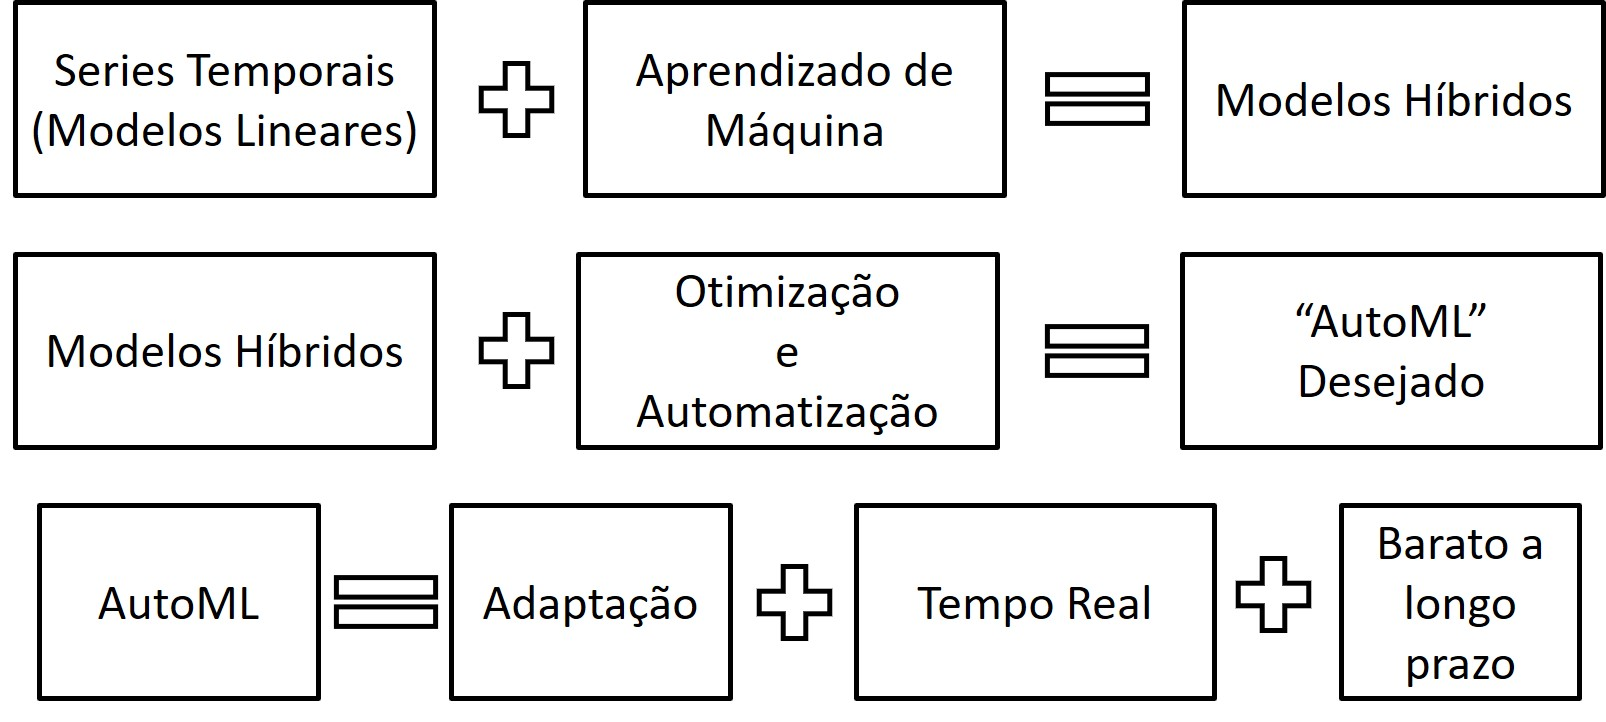
\includegraphics[width=\textwidth]{Figuras/introducao/intro_nutshell.jpg}
    \source{Autor.}
    \label{fig:cap1_intro_nutshell}
\end{figure}

Este trabalho faz parte de um projeto maior de pesquisa e desenvolvimento (P\&D) Financiado pela CHESF(Companhia Hidrelétrica do São Francisco) e Regulado pela ANEEL (Agência Nacional de Energia Elétrica), que será aplicado na subestação (SE) de Messias localizada na região metropolitana de Maceió - AL.

\section{Estrutura do projeto}

A organização das seções deste trabalho se dá da seguinte forma. Primeiramente serão apresentados os objetivos no capítulo \ref{cap:objetivos}, após isto será feita uma análise do estado da arte no capítulo \ref{cap:estado_da_arte}, depois disso são apresentados no capítulo \ref{cap:materiais_e_metodos} materiais e métodos, apresentando a teoria da previsão de séries temporais utilizando modelos lineares \ref{sec:series_temp}, dados que serão utilizados \ref{sec:dados_prep} e modelos propostos \ref{sec:auto_ml}. São apresentados em seguida, cronograma \ref{cap:cronograma}, resultados \ref{cap:resultados} contendo preliminares e esperados, e por fim conclusões \ref{cap:conclusoes}.